\begin{frame}
  \frametitle{Review: Parallel Combination}

  Parallel combination of two systems looks like this:
  \vspace*{3mm}

  \centerline{\begin{tikzpicture}
      \node[dspnodeopen,dsp/label=right] (y) at (2,0) {$y[n]$};
      \node[dspadder] (adder) at (1,0) {}  edge[dspflow] (y);
      \node[coordinate] (y1) at (1,1) {}  edge[dspline] (adder);
      \node[coordinate] (y2) at (1,-1) {}  edge[dspline] (adder);
      \node[dspsquare] (h1) at (0,1) {$H_1(z)$}  edge[dspline] (y1);
      \node[dspsquare] (h2) at (0,-1) {$H_2(z)$}  edge[dspline] (y2);
      \node[coordinate] (x1) at (-1,1) {}  edge[dspconn] (h1);
      \node[coordinate] (x2) at (-1,-1) {}  edge[dspconn] (h2);
      \node[dspnodefull] (xsplit) at (-1,0) {} edge[dspline](x1) edge[dspline](x2);
      \node[dspnodeopen,dsp/label=left] (x) at (-2,0) {$x[n]$} edge[dspline] (xsplit);
  \end{tikzpicture}}
  Suppose that we know each of the systems separately:
  \[
  H_1(z)=\frac{1}{1-p_1z^{-1}},~~~~~
  H_2(z)=\frac{1}{1-p_2z^{-1}}
  \]
  Then, to get $H(z)$, we just  have to add:
  \[
  H(z) = \frac{1}{1-p_1z^{-1}}+\frac{1}{1-p_2z^{-1}}= \frac{2-(p_1+p_2)z^{-1}}{1-(p_1+p_2)z^{-1}+p_1p_2z^{-2}}
  \]
\end{frame}


\begin{frame}
  \frametitle{Understanding the Impulse Response of a Second-Order IIR}

  In order to {\bf understand} the impulse response, maybe we should
  invent some more variables.  Let's say that
  \[
  p_1 = e^{-\sigma_1+j\omega_1},~~~p_1^* = e^{-\sigma_1-j\omega_1}
  \]
  where $\sigma_1$ is the half-bandwidth of the pole, and $\omega_1$
  is its center frequency.  The partial fraction expansion gave us the constant
  \begin{displaymath}
    C_1 = \frac{p_1}{p_1-p_1^*}= \frac{p_1}{e^{-\sigma_1}\left(e^{j\omega_1}-e^{-j\omega_1}\right)}
    = \frac{e^{j\omega_1}}{2j\sin(\omega_1)}
  \end{displaymath}
  whose complex conjugate is
  \[
  C_1^* = -\frac{e^{-j\omega_1}}{2j\sin(\omega_1)}
  \]
\end{frame}

\begin{frame}
  \frametitle{Impulse Response of a Second-Order IIR}

  Plugging in to the impulse response, we get
  \begin{align*}
    h[n] &= \frac{1}{2j\sin(\omega_1)}
    \left(e^{j\omega_1}e^{(-\sigma_1+j\omega_1)n}-e^{-j\omega_1}e^{(-\sigma_1-j\omega_1)n}\right)u[n]\\
    &= \frac{1}{2j\sin(\omega_1)}e^{-\sigma_1n}\left(e^{j\omega_1(n+1)}-e^{-j\omega_1(n+1)}\right)u[n]\\
    &= \frac{1}{\sin(\omega_1)} e^{-\sigma_1n}\sin(\omega_1(n+1)) u[n]
  \end{align*}
\end{frame}

\begin{frame}
  \frametitle{Impulse Response of a Second-Order IIR}

  \[
  h[n] = \frac{1}{\sin(\omega_1)} e^{-\sigma_1n}\sin(\omega_1(n+1)) u[n]
  \]
  \centerline{\includegraphics[height=2.5in]{exp/dampedimpulse49.png}}
\end{frame}


\begin{frame}
  \frametitle{Example: Stable Resonator}

  Just to make it concrete, let's choose $\omega_1=\frac{\pi}{4}$, and
  $e^{-\sigma_1}=0.9$, so the difference equation is
  \[
  y[n] = x[n] + 0.9\sqrt{2} y[n-1] - 0.81 y[n-2]
  \]
  If we plug $x[n]=\delta[n]$ into this equation, we get
  \begin{align*}
    y[0] &= 1\\
    y[1] &= 0.9\sqrt{2}\\
    y[2] &= (0.9\sqrt{2})^2 - 0.81 = 0.81\\
    y[3] &= (0.9\sqrt{2})(0.81)-(0.81)(0.9\sqrt{2})=0\\
    y[4] &= -(0.81)^2\\
    y[5] &= -(0.9\sqrt{2})(0.81)^2\\
    &\vdots
  \end{align*}
\end{frame}

%%%%%%%%%%%%%%%%%%%%%%%%%%%%%%%%%%%%%%%%%%%%
\section[Real-World]{Real-world resonators}
\setcounter{subsection}{1}

\begin{frame}
  \frametitle{Real-world damped resonators}

  In the real world, many systems resonate.  All of them lose energy gradually, so
  they are all damped.  Examples include:
  \begin{itemize}
  \item Earthquakes are caused when a geological fault shifts (a unit step),
    causing the nearby crust to shake back and forth
  \item Suddenly changing the voltage on an antenna will cause its current
    to resonate, generating electromagnetic waves in the air
  \item Plucking a guitar string causes it to resonate
  \item When you clap in a shower stall, you can hear decaying sine waves
    at its resonant frequencies
  \item When your vocal folds close, the air in your mouth resonates
  \end{itemize}
\end{frame}

\begin{frame}
  \frametitle{Speech is made up of Damped Sinusoids}

  \centerline{\includegraphics[width=4.5in]{exp/speechwave.png}}
\end{frame}

\begin{frame}
  \frametitle{Speech is made up of Damped Sinusoids}

  Your vocal tract has an infinite number of resonant frequencies, all
  of which ring at once:
  \[
  H(z)  = \prod_{k=1}^\infty \frac{1}{(1-p_kz^{-1})(1-p_k^*z^{-1})}
  \]
  There are an infinite number, but most are VERY heavily damped, so
  usually we only hear the first three or four.
\end{frame}

\begin{frame}
  \frametitle{Center Freqs of First Two Poles Specify the Vowel\\\begin{tiny}(Peterson \& Barney, 1952)\end{tiny}}

  \centerline{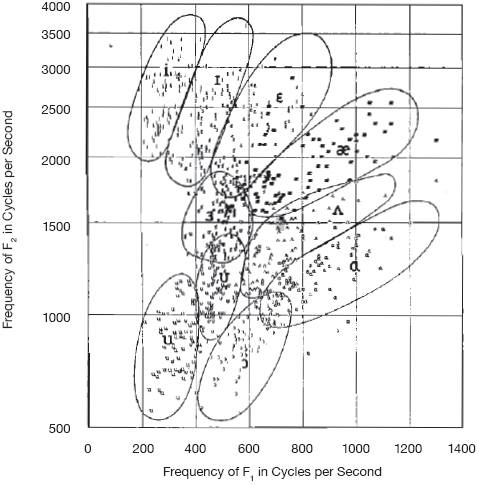
\includegraphics[height=3in]{pg23.jpg}}
\end{frame}

\begin{frame}
  \frametitle{First Formant Resonator}

  When you look at a speech waveform, $x[n]$, most of what you see is
  the first resonance, called the ``first formant.''  Its resonant
  frequency is roughly $400\le F_1\le 800$ usually, so at $F_s=16000$Hz
  sampling frequency, we get
  \[
  \omega_1 = \frac{2\pi F_1}{F_S} \in \left[\frac{\pi}{20},\frac{\pi}{10}\right]
  \]
  Its bandwidth might be about $B_1\approx 400$Hz, so
  \[
  \sigma_1 = \frac{1}{2}\left(\frac{2\pi B_1}{F_s}\right) \approx \frac{\pi}{40}
  \]
\end{frame}

\begin{frame}
  \frametitle{First Formant Frequency and  Bandwidth in the Waveform}

  \centerline{\includegraphics[width=4.5in]{exp/speechwaves.png}}
\end{frame}


\begin{frame}
  \frametitle{First Formant Frequency and  Bandwidth in the Spectrum}

  \centerline{\includegraphics[width=4.5in]{exp/speechspecs.png}}
\end{frame}

    
\begin{frame}
  \frametitle{Magnitude Response at $\omega=\omega_1\pm\epsilon$}
  \begin{itemize}
  \item There are two poles, one at $\omega_1$, one at $-\omega_1$.
  \item The pole at $-\omega_1$ is very far away from $\omega\approx +\omega_1$.
    In fact, over the whole range $\omega=\omega_1\pm\epsilon$, this distance
    remains approximately constant:
    \begin{align*}
      |e^{j\omega}-p_1^*|&= |e^{j(\omega_1\pm\epsilon)}-e^{-\sigma_1-j\omega_1}|\\
      &\approx |e^{j\omega_1}-e^{-j\omega_1}|\\
      &= 2|\sin(\omega_1)|
    \end{align*}
  \end{itemize}
\end{frame}  

\begin{frame}
  \frametitle{Magnitude Response at $\omega=\omega_1\pm\epsilon$}

  Now let's suppose $p_1=e^{-\sigma_1+j\omega_1}$, and
  $p_2=p_1^*=e^{-\sigma_1-j\omega_1}$.  Consider what happens when
  $\omega=\omega_1\pm\epsilon$ for small values of $\epsilon$.
  \begin{itemize}
  \item There are two poles, one at $\omega_1$, one at $-\omega_1$.
  \item The pole at $-\omega_1$ is very far away from $\omega\approx +\omega_1$.
    In fact, over the whole range $\omega=\omega_1\pm\epsilon$, this distance
    remains approximately constant:
    \begin{align*}
      |e^{j\omega}-p_1^*|&= |e^{j(\omega_1\pm\epsilon)}-e^{-\sigma_1-j\omega_1}|\\
      &\approx |e^{j\omega_1}-e^{-j\omega_1}|\\
      &= 2|\sin(\omega_1)|
    \end{align*}
  \end{itemize}
\end{frame}  

